\section{Convexity, Lipschitzness, and Smoothness}
\frame{\tableofcontents[currentsection, hideothersubsections]}

\begin{frame}
\frametitle{Convexity: Convex sets}

\begin{figure}
    \centering
    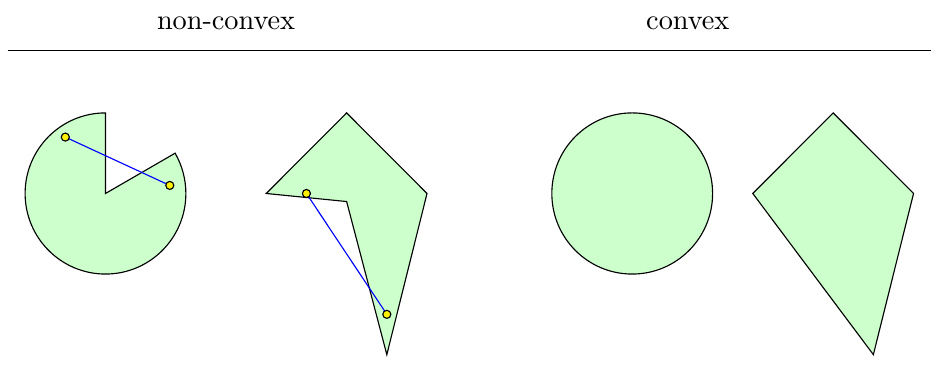
\includegraphics[scale=0.35]{cvx_noncvx}
\end{figure}

\begin{figure}
    \centering
    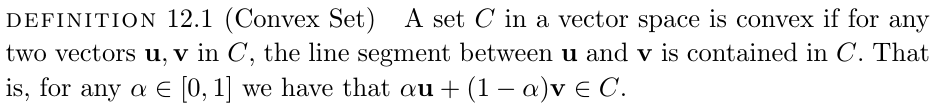
\includegraphics[scale=0.4]{cvx_set}
\end{figure}

\end{frame}

\begin{frame}
\frametitle{Convexity: Convex functions}

\begin{figure}
    \centering
    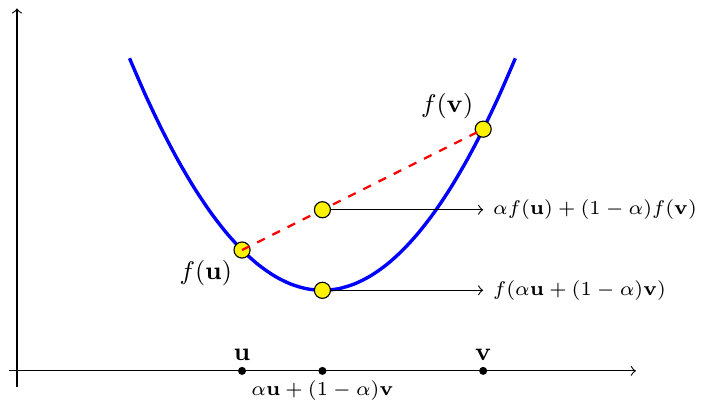
\includegraphics[scale=0.35]{cvx_fn}
\end{figure}

\begin{figure}
    \centering
    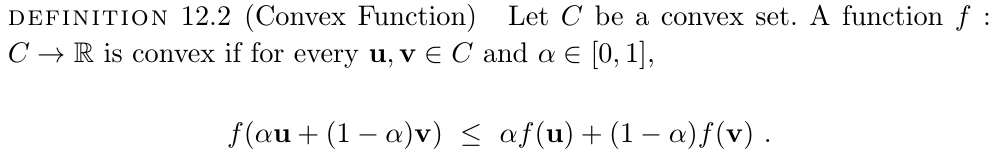
\includegraphics[scale=0.4]{cvx_fn_def}
\end{figure}

\end{frame}

\begin{frame}
\frametitle{Convexity: Convex functions}

Properties of convex fn:
\begin{itemize}
    \item  every local minimum is also a global minimum
    \item  for every $\mathbf{w}$ we can construct a tangent to $f$
    at $\mathbf{w}$ that lies below $f$ everywhere.
    If f is differentiable, this tangent is the linear function
    % $l(u) = f(w) + h∇f (w), u − wi$
\end{itemize}

\begin{figure}
    \centering
    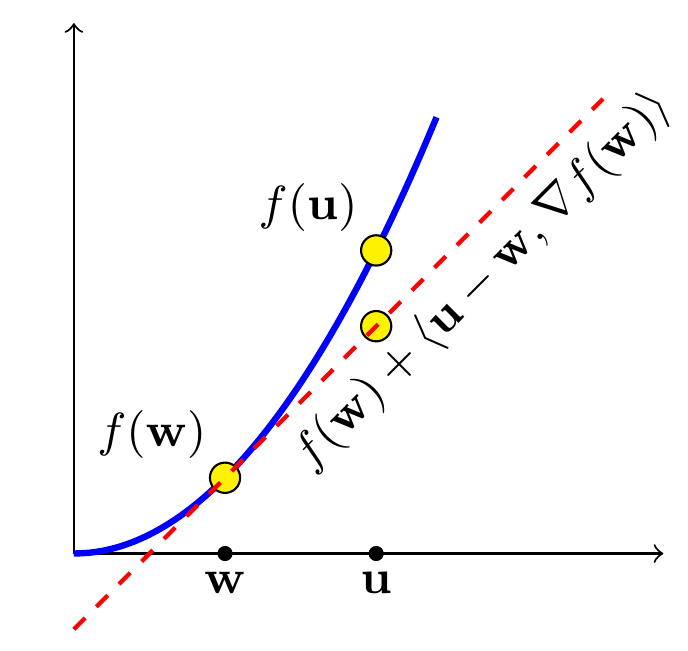
\includegraphics[scale=0.25]{cvx_fn_tangent}
\end{figure}

\end{frame}

\begin{frame}
\frametitle{Convexity: Convex functions}

\begin{figure}
    \centering
    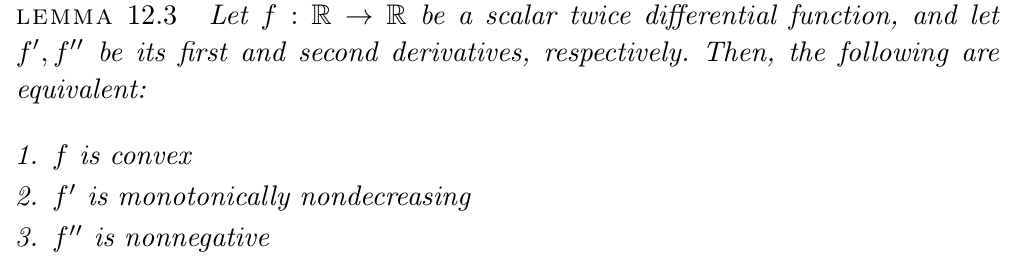
\includegraphics[scale=0.35]{lemma_12_3}
\end{figure}

\noindent\makebox[\linewidth]{\rule{\paperwidth}{0.4pt}}

\begin{figure}
    \centering
    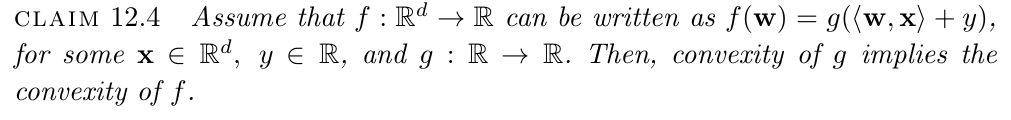
\includegraphics[scale=0.375]{claim_12_4}
\end{figure}

\noindent\makebox[\linewidth]{\rule{\paperwidth}{0.4pt}}

\begin{figure}
    \centering
    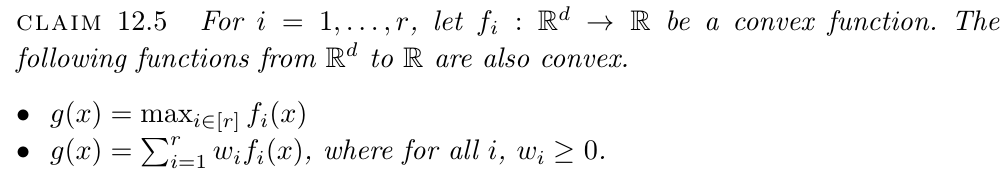
\includegraphics[scale=0.375]{claim_12_5}
\end{figure}

\end{frame}


\begin{frame}
\frametitle{Lipschitzness}
\begin{figure}
    \centering
    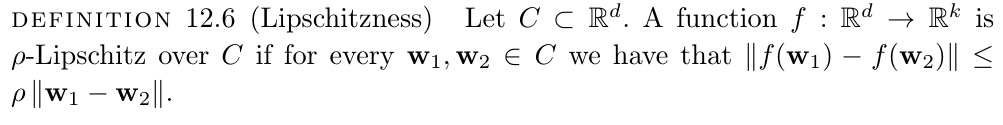
\includegraphics[scale=0.45]{def_12_6}
\end{figure}

Properties:
\begin{itemize}
    \item a Lipschitz function can \textbf{not} change too fast
    \item if the derivative of $f$ is everywhere bounded (in absolute value) by $\rho$,
        then the function is $\rho$-Lipschitz.
    \item \textbf{composition} of Lipschitz functions \textbf{preserves} Lipschitzness.
\end{itemize}

\end{frame}


\begin{frame}
\frametitle{Smoothness}
\begin{figure}
    \centering
    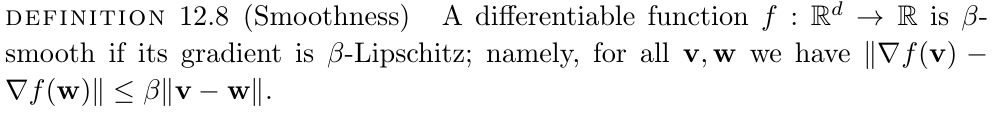
\includegraphics[scale=0.45]{def_12_8}
\end{figure}

Properties:
\begin{itemize}
    \item when a function is \textbf{both} convex and smooth,\\
        we have both \textbf{upper and lower bounds} on the difference between
        the function and its first order approximation.
    \item a \text{composition} of a smooth scalar function over a linear function \textbf{preserves} smoothness.
    \begin{figure}
        \centering
        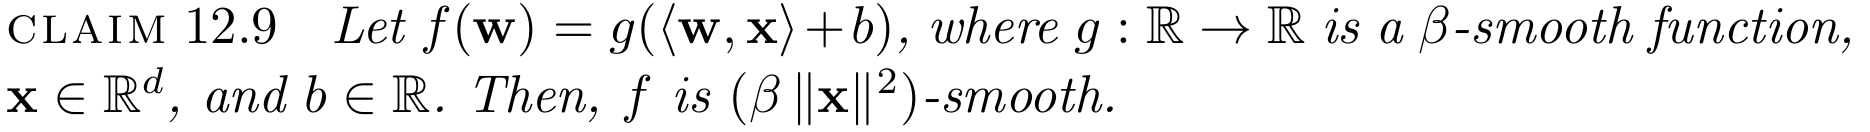
\includegraphics[scale=0.225]{claim_12_9}
    \end{figure}
\end{itemize}

\end{frame}
